\documentclass[12pt,a4paper]{article}
\usepackage[utf8]{inputenc}
\usepackage[czech]{babel}
\usepackage[T1]{fontenc}
\usepackage{amsmath}
\usepackage{amsfonts}
\usepackage{amssymb}
\usepackage{graphicx}
\usepackage[unicode=true]{hyperref}
\usepackage{index}
\usepackage{listings}
\usepackage{url}
\usepackage{enumitem}
\usepackage[left=2cm,right=2cm,top=2cm,bottom=2cm]{geometry}
\author{Roman Ondráček}
\title{Projekt IUS - Model informačního systému}
\lstset{inputencoding=utf8}
% Řádkování 1,5
\renewcommand{\baselinestretch}{1.5}
\begin{document}

% Vynechání číslování
\pagestyle{empty}

\begin{center}


\includegraphics[height = 96pt]{img/FIT_barevne_CMYK_CZ.pdf} \\

\begin{LARGE}
\textbf{Vysoké učení technické v Brně} \\
\end{LARGE}

\begin{large}
Fakulta informačních technoligií \\
Úvod do softwarového inženýrství \\
2018~/~2019 \\
\end{large}

\vspace{128pt}

\begin{huge}
\textbf{Zadání č.~60. Food and Activity Tracker} \\
\end{huge}

\begin{large}
Projekt IUS - Model informačního systému \\
\end{large}

\end{center}

\vfill

Roman Ondráček (xondra58) \hfill \today

% Povolení číslování
\pagestyle{plain}

\newpage

\section*{Zadání}

Jelikož jsi jistě aktivní sportovec, měl bys rád přehled o~tom, kolik energie spálí a přijme tvé tělo. A tak se rozhodneš vytvořit IS, kde by si každý, kdo poskytne informace o~svém pohlaví, cílové hmotnosti a bazálním metabolismu, mohl každý měsíc ukládat informace o~své aktuální hmotnosti, výšce, obvodu hrudníku, obvodu pasu, stehen a lýtek, aby měl přehled o~tom, zda jeho svalová hmota narůstá. Díky Food and Activity Trackeru si tak může zobrazit graf a zjistit, jak si vedl za poslední měsíc, půl roku nebo rok. V rámci Food and Activity Trackeru si může vytvářet záznam o~snědených jídlech (snídaně, oběd, svačiny, atd.) v~rámci jednoho dne, a to buď přidáním poměrné části uloženého receptu nebo jako seznam jednotlivých potravin z~databáze potravin určitého množství. Potraviny i recepty do databáze vkládají samotní uživatelé aplikace. Zároveň si mohou vytvářet seznam svých oblíbených receptů, ať už svých, anebo ostatních uživatelů. Uživatel se díky aplikaci může dozvědět svůj celkový příjem a výdej energie a celkový příjem bílkovin, sacharidů, tuků a vlákniny během dne. U jednotlivých potravin se dozví informace o jejich nutričních hodnotách a popis. Aby si uživatel mohl připravit recept, musí vědět, jaké ingredience a v~jakém množství k~přípravě jídla potřebuje, postup, jeho obtížnost, dobu přípravy, počet porcí a jelikož si hlídá svůj příjem, tak také informaci o~kalorické hodnotě jídla a množství bílkovin, sacharidů, vlákniny a tuků. Aby snědenou energii nějak spálil, musí se také věnovat pravidelně nějakému sportovní aktivitě a o~každé takové aktivitě během dne si v rámci záznamu svého denního příjmu/výdeji vede záznam. V~databázi sportů si vyhledá aktivitu, kterou provozoval a podle doby trvání, své hmotnosti a výšky se pak vytvoří záznam o~spálených kaloriích. \\

\newpage

\section{Model případů užití}

\vspace*{\fill}
\begin{center}
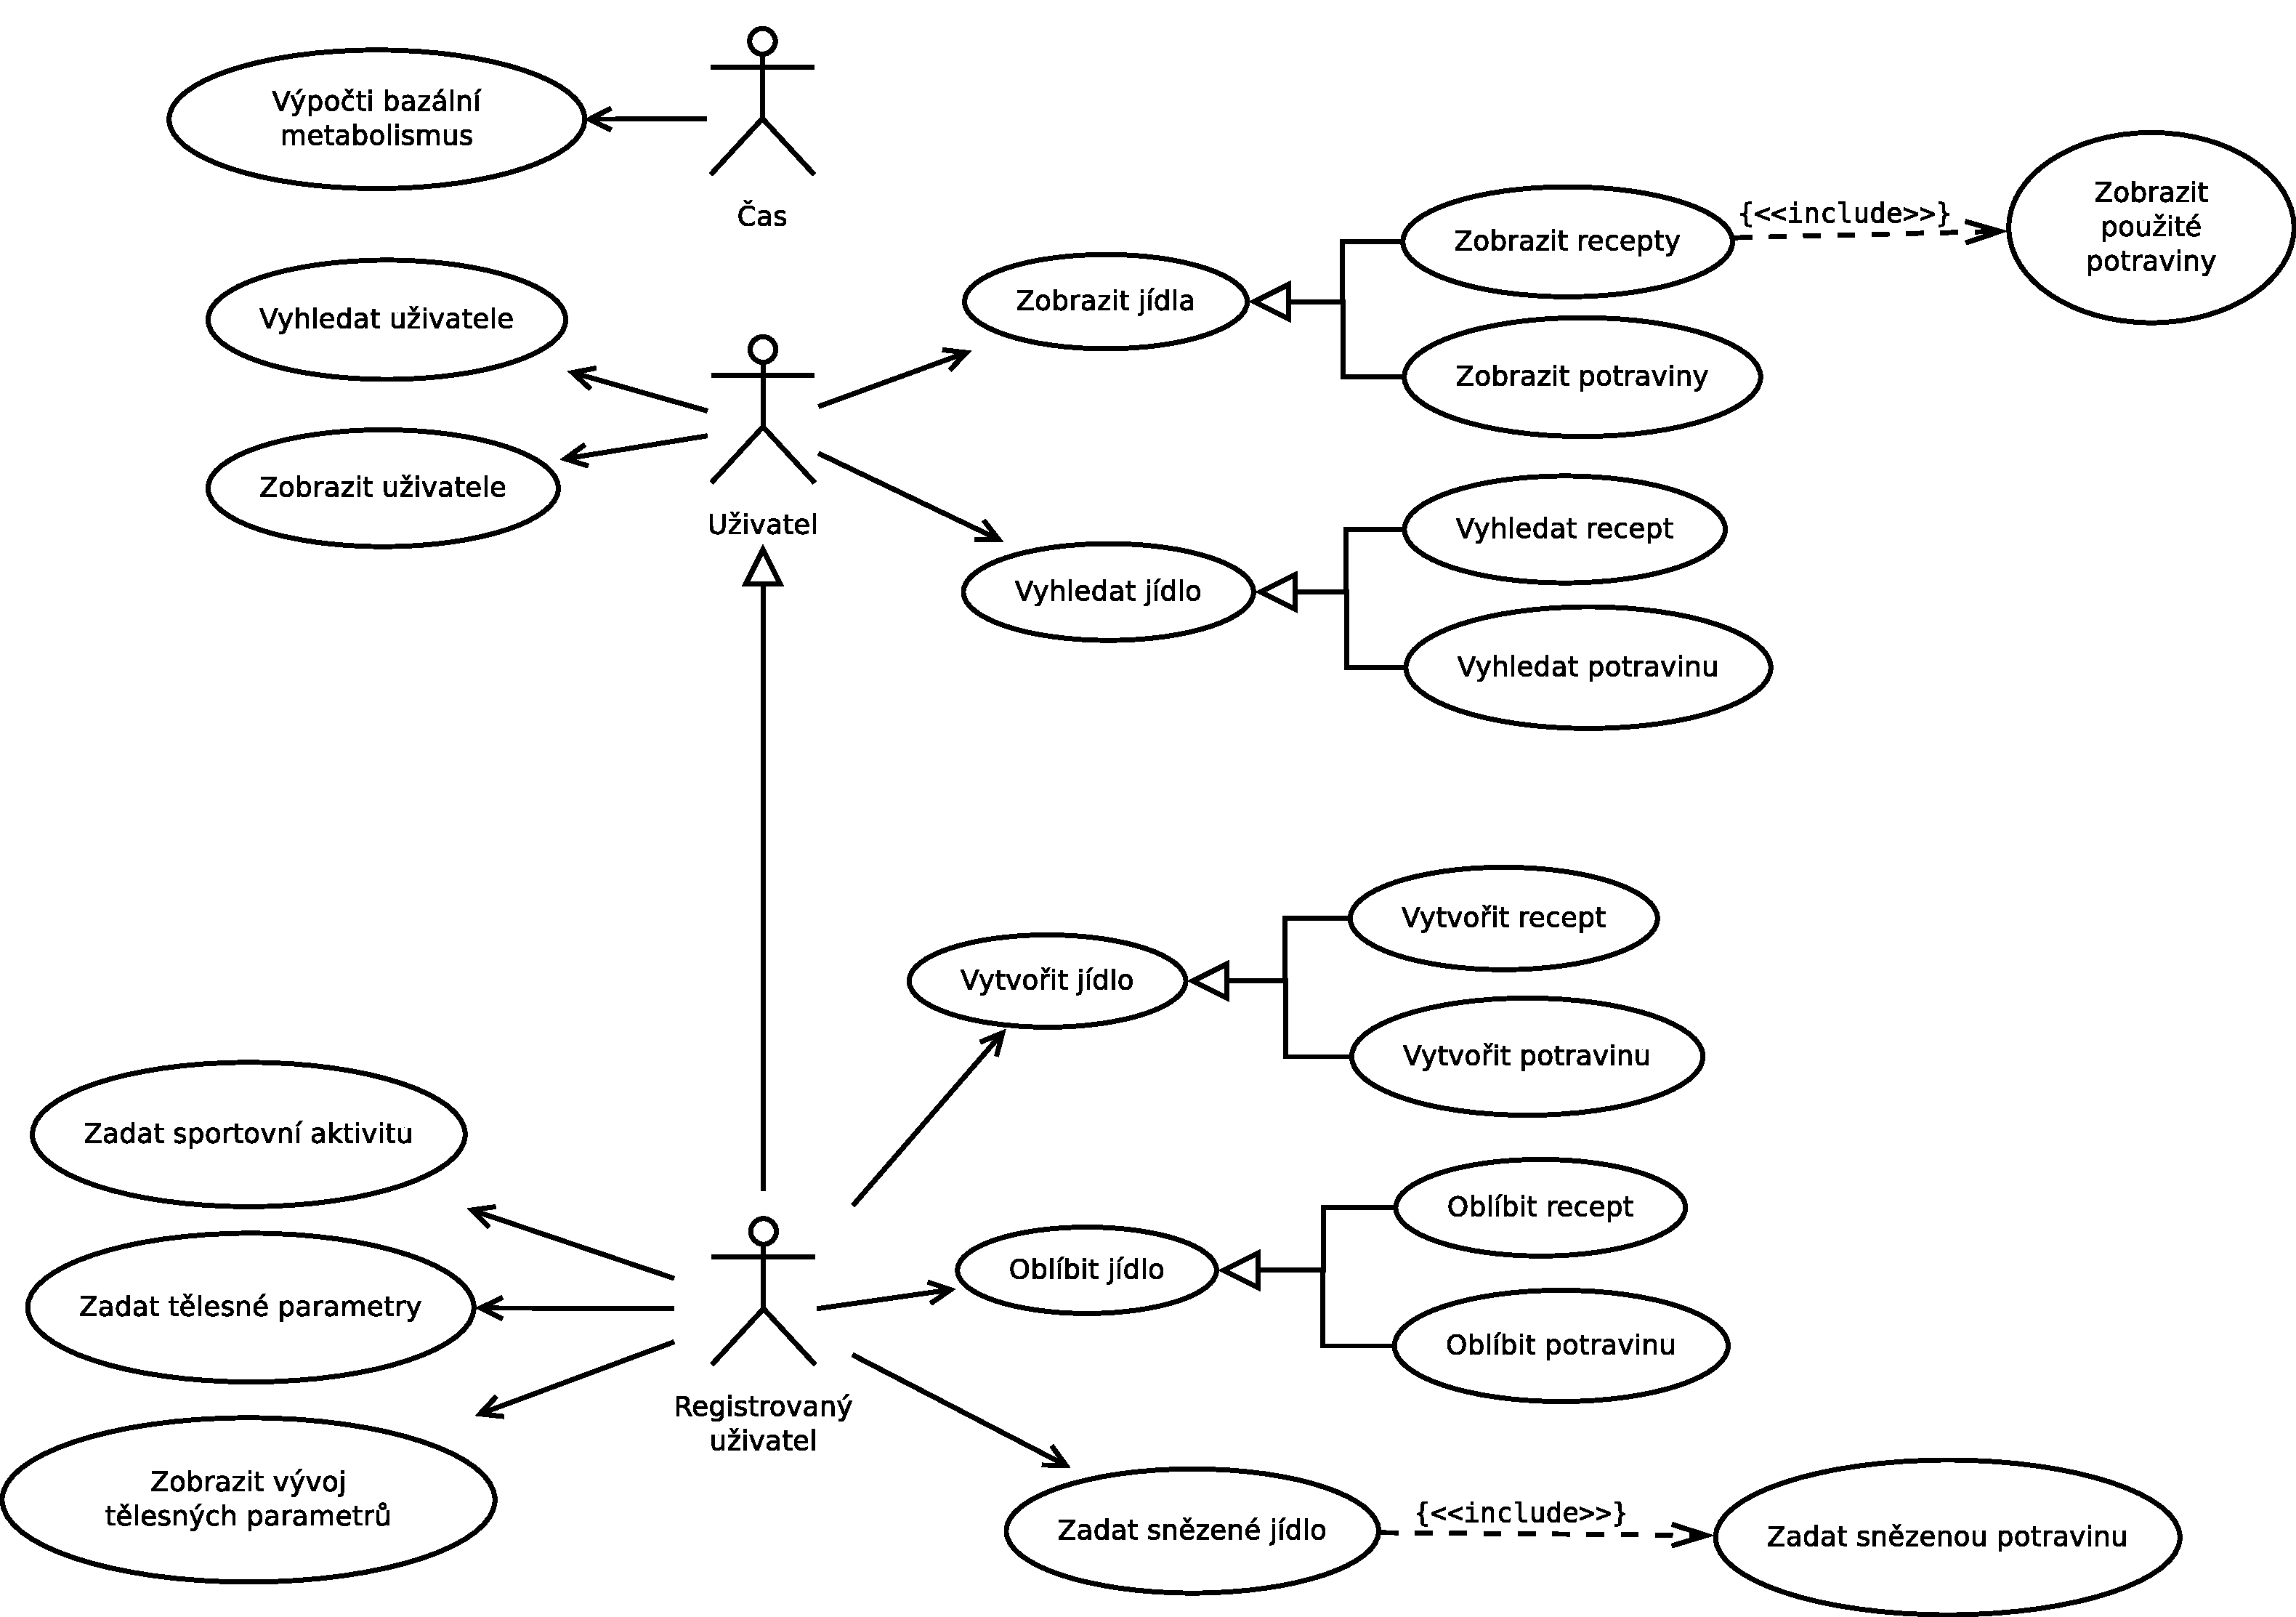
\includegraphics[angle=90,origin=c,height = \textwidth]{img/use-case.pdf} \\
\end{center}
\vspace*{\fill}

\newpage

\section{ER diagram}

\vspace*{\fill}
\begin{center}
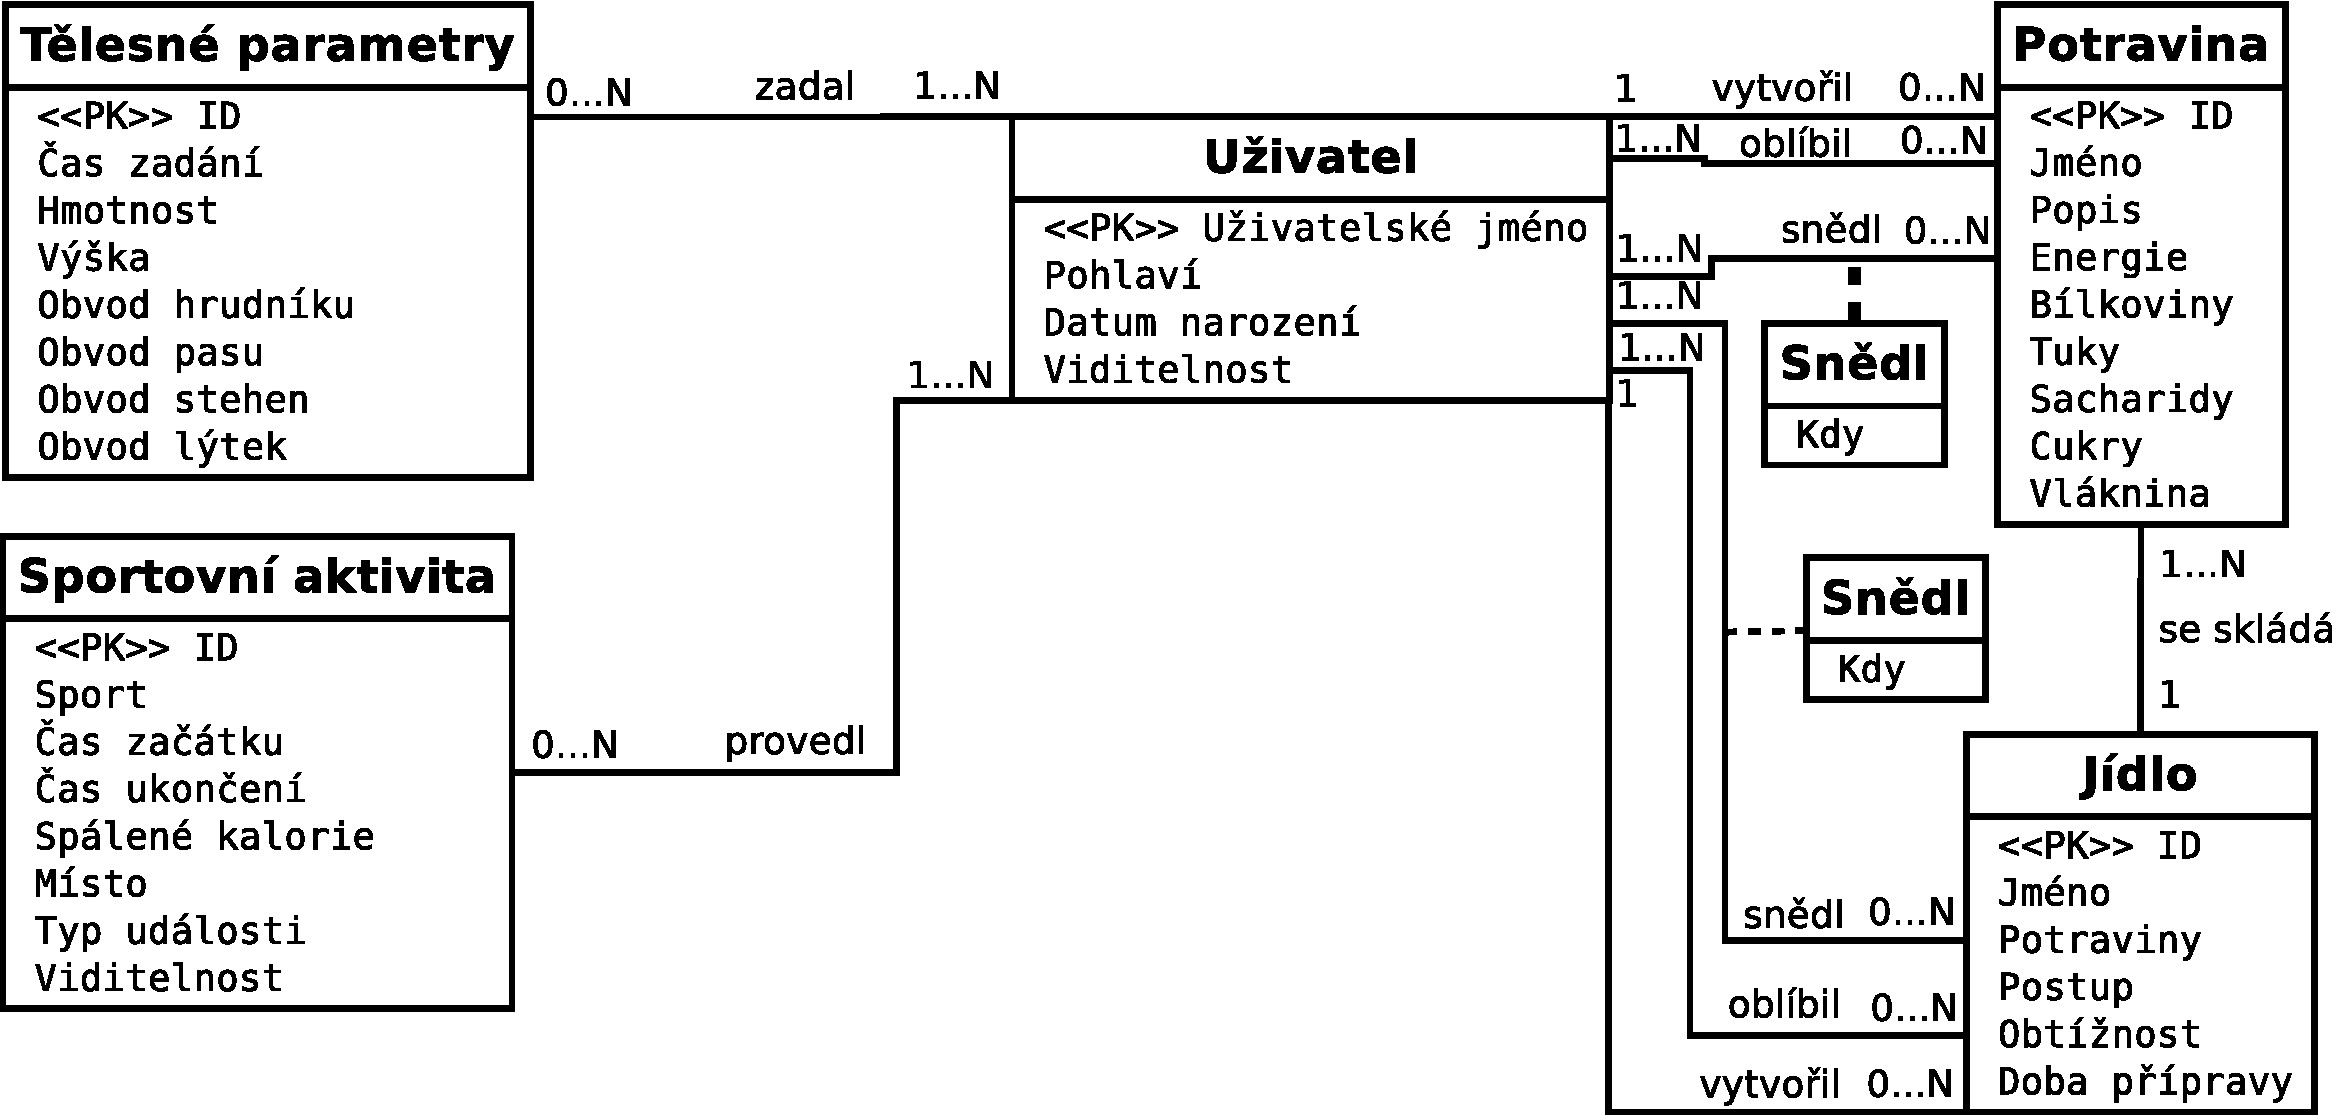
\includegraphics[angle=90,origin=c,height = \textwidth]{img/er.pdf} \\
\end{center}
\vspace*{\fill}

\end{document}
